%%%%%%%%%%%%%%%%%%%%%%%%%%%%%%%%%%%%%%%%%%%%%%%%%%%%%%%%%%%%%%%%%%%%
%% I, the copyright holder of this work, release this work into the
%% public domain. This applies worldwide. In some countries this may
%% not be legally possible; if so: I grant anyone the right to use
%% this work for any purpose, without any conditions, unless such
%% conditions are required by law.
%%%%%%%%%%%%%%%%%%%%%%%%%%%%%%%%%%%%%%%%%%%%%%%%%%%%%%%%%%%%%%%%%%%%

\documentclass[
  digital, %% This option enables the default options for the
           %% digital version of a document. Replace with `printed`
           %% to enable the default options for the printed version
           %% of a document.
  table,   %% Causes the coloring of tables. Replace with `notable`
           %% to restore plain tables.
% * <michalsindelar03@gmail.com> 2016-04-19T17:32:28.735Z:
%
% ^.
  lof,     %% Prints the List of Figures. Replace with `nolof` to
           %% hide the List of Figures.
  lot,     %% Prints the List of Tables. Replace with `nolot` to
           %% hide the List of Tables.
  %% More options are listed in the user guide at
  %% <http://mirrors.ctan.org/macros/latex/contrib/fithesis/guide/mu/fi.pdf>.
]{fithesis3}
%% The following section sets up the locales used in the thesis.
\usepackage[resetfonts]{cmap} %% We need to load the T2A font encoding
\usepackage[T1,T2A]{fontenc}  %% to use the Cyrillic fonts with Russian texts.
\usepackage[
  main=czech, %% By using `czech` or `slovak` as the main locale
                %% instead of `english`, you can typeset the thesis
                %% in either Czech or Slovak, respectively.
  english, german, russian, slovak %% The additional keys allow
]{babel}        %% foreign texts to be typeset as follows:
%%
%%   \begin{otherlanguage}{german}  ... \end{otherlanguage}
%%   \begin{otherlanguage}{russian} ... \end{otherlanguage}
%%   \begin{otherlanguage}{czech}   ... \end{otherlanguage}
%%   \begin{otherlanguage}{slovak}  ... \end{otherlanguage}
%%
%% For non-Latin scripts, it may be necessary to load additional
%% fonts:
\usepackage{paratype}
\def\textrussian#1{{\usefont{T2A}{PTSerif-TLF}{m}{rm}#1}}
%%
%% The following section sets up the metadata of the thesis.
\thesissetup{
    date          = \the\year/\the\month/\the\day,
    university    = mu,
    faculty       = fi,
    type          = bc,
    author        = Michal Šindelář,
    gender        = m,
    advisor       = RNDr. Vladimír Ulman\, Ph.D.,
    title         = {Optické měření srdečního pulsu z~krátkého kamerového záznamu},
    TeXtitle      = {Optické měření srdečního pulsu z~krátkého kamerového záznamu},
    keywords      = {Digitální zpracování obrazu, určení tepu z~optického záznamu, Eulerian magnification, fotopletysmografie},
    TeXkeywords   = {Digitální zpracování obrazu, určení tepu z~optického záznamu, Eulerian magnification},
}
\thesislong{abstract}{
  Cílem projektu je vytvořit aplikaci, která nabídne vytvoření krátkého kamerového záznamu obličeje, přehrání záznamu a současně vyobrazení srdečního tepu (například poblikávání ikonky v~detekovaném rytmu). Srdeční tep bude detekován pouze na základě analýzy obrazu z~kamery. Metoda je založena na zdůraznění slabé, okem těžko pozorovatelné fluktuace barevného odstínu kůže vlivem přítomnosti nebo nepřítomnosti krve.

Těžiště práce je nalezení a zrealizovaní procedury zachycení a zpracování snímků videa. Konkrétně bude potřeba programově zajistit stabilní snímací podmínky, optimalizovat snímané video pro další zpracování, spustit existující program na zesílení barevných fluktuací (nebo ho vytvořit znovu), detekovat pulsování barev ve zpracované sekvenci a určit tepovou rychlost. Vše se potom zabalí do GUI aplikace. Ideální výsledek práce je online zpracování videa, to je však poměrně ambiciózní.

Práce buď využije hotovou implementaci původních autorů této techniky a vloží ji do hotové aplikace, nebo celý postup naprogramuje samostatně (s~přihlédnutím na kontext aplikace) v~libovolném programovacím jazyku.


\begin{otherlanguage}{english}
Literatura: Hao-Yu Wu, Michael Rubinstein, Eugene Shih, John Guttag, Fredo Durand and William T. Freeman. Eulerian Video Magnification for Revealing Subtle Changes in the World. In ACM Transactions on Graphics (Proc. SIGGRAPH 2012), 31, 4. 2012.
\end{otherlanguage}

}
\thesislong{thanks}{
Rád bych především poděkoval RNDr. Vladimíru Ulmanovi\, Ph.D. za vedení mé bakalářské práce, odborné rady a ochotu.

Dále děkuji rodině, kamarádům a všem, kteří mě při studiu a tvorbě práce podporovali. Především potom rodičům, kteří navíc souhlasili se zveřejněním fotografií demonstrující měření využitá v~práci.
}
%% The following section sets up the bibliography.
\usepackage{csquotes}
\usepackage[              %% When typesetting the bibliography, the
  backend=biber,          %% `numeric` style will be used for the
  style=numeric,          %% entries and the `numeric-comp` style
  citestyle=numeric-comp, %% for the references to the entries. The
  sorting=none,           %% entries will be sorted in cite order.
  sortlocale=auto         %% For more unformation about the available
]{biblatex}               %% `style`s and `citestyles`, see:
%% <http://mirrors.ctan.org/macros/latex/contrib/biblatex/doc/biblatex.pdf>.
\addbibresource{example.bib} %% The bibliograpic database within
\addbibresource{resources.bib} %% The bibliograpic database within
                          %% the file `example.bib` will be used.
\usepackage{makeidx}      %% The `makeidx` package contains
\makeindex                %% helper commands for index typesetting.
%% These additional packages are used within the document:
\usepackage{paralist}
\usepackage{amsmath}
\usepackage{amsthm}
\usepackage{amsfonts}
\usepackage{url}
\usepackage{menukeys}
\usepackage{csvsimple, longtable, booktabs}
\usepackage{lscape}

\begin{document}

\chapter{Úvod}
\section{Digitální zpracování obrazu}
Digitální zpracování obrazu je vědní obor informatiky, který nabízí techniky pro zkoumání digitálního obrazu za účelem zisku informací, či vyprodukování \emph{vylepšeného} obrazu. Typickým odvětvím, ve kterém nachází digitální zpracování obrazu uplatnění je medicína. 

V~medicíně se využívá např. pro zobrazení výsledků rentgenu, magnetické rezonance a dalších. Tato práce se bude zabývat dalším potenciálním využitím digitálního zpracování obrazu konkrétně pro zkoumání tepové frekvence lidského těla z~optického záznamu. 

\section{Tepová frekvence}
Každý člověk má tep, který je vyvolán vypuzením krve ze srdeční komory do aorty a následně dále do těla. Tep odpovídá počtu úderů srdce za minutu. Jeho hodnota se liší člověk od člověka. 

Klidová tepová frekvence je jedním ze základních rutin měření v~medicínské péči. Tato frekvence odpovídá situaci, kdy srdce vypuzuje minimální množství krve. Pro správné měření musí být člověk zdravý a ve fyzickém i psychickém klidu.

% TODO: Rozmezí -> PRACOVNÍ INTERVAL
% Obrázek velký o O
% Zkontrolovat odkazy na publikace
Pro určení pracovního intervalu tepu, který má smysl zkoumat práce využívá \emph{Národní zdravotní statistické záznamy} \cite{national-health-statistics-reports} měřené roku 2011 v~USA. Klidový tep ovlivňuje více faktorů jako fyzická kondice, zdraví a především věk. Pro novorozence do jednoho roku je průměrná frekvence 129 tepů/min zatímco pro dospělé už jen 72 tepů/min.

Srdeční frekvence nižší než 60 tepů se považuje za abnormálně pomalou a označuje se jako bradykardie. Hraniční hodnota se ovšem vždy vztahuje i k~věkové a výkonnostní kategorii, např. u~sportovců je běžné mít sníženou klidovou frekvenci i pod 60. Opakem bradykardie je tachykardie\footnote{Blíže viz \url{http://www.heart.org/HEARTORG/Conditions/Arrhythmia/AboutArrhythmia/Tachycardia-Fast-Heart-Rate_UCM_302018_Article.jsp}}, která je u~dospělých obvykle diagnostikována nad 100 tepů/min (u~dospělých).

Práce vylučuje abnormální případy a zaměří se na interval 55-180 tepů/min, kterým bude pokryto vše kromě extrémně nízkých tepů způsobených bradykardií, či profesionálním tréninkem vrcholových sportovců. Pracovní interval bude stěžejní při odhalování výsledné frekvence z~videa. Rozšíření intervalu o~ještě nižší frekvence je problematické a většinou vede k~nekorektním výsledkům.

Srdeční tep můžeme znázornit pomocí přístroje EKG. EKG je zkratka pro vyšetřovací metodu zvanou elektrokardiografie, kdy přístroj snímá elektrické aktivity srdce. Zanáší je do grafu zvaného elektrokardiogram (viz Obrázek \ref{fig:electrocardiograph}) a umožňuje hodnocení aktivity srdce\footnote{Blíže viz \url{http://emedicine.medscape.com/article/1894014-overview>}}. V~elektrokardiogramu odpovídají intervaly mezi jednotlivými lokálními minimy tepové frekvenci srdce.

\begin{figure}
  \begin{center}
    \includegraphics[width=120mm]{images/electrocardiograph.png}
  \end{center}
  \caption{Ilustrace ideálního elektrokardiogramu.}
  \label{fig:electrocardiograph}
\end{figure}

\section{Cíle aplikace}
Cílem této aplikace je využití fyziologických vlastností proudění krve v~těle za účelem určení tepové frekvence pouze ze záznamu obličeje. Po určení bude tep vhodným způsobem vyobrazen uživateli.

Aplikace bude pracovat buď s~vloženým záznamem, nebo pro záznam bude využívat přímo webkameru zařízení, na kterém poběží. Při snímání pomocí levnějších (běžných) webkamer se dají očekávat problémy s~proměnlivou vzorkovací frekvencí a také s~automatickou změnou expozice.

Aplikace bude mít celkem 3 různé režimy:
\begin{enumerate}
  \item \emph{Statický} režim při dodaném záznamu \\
    V~tomto režimu uživatel dodá aplikaci hotový záznam. Ta bude zpracovávat záznam celý a výpočet skončí až po zpracování celého videa. Tento režim by měl (v~závislosti na délce videa) vést k~nejlepším výsledkům, zároveň je ale časově nejnáročnější a prodleva bez interakce s~uživatelem je po celou dobu zpracování. Dále v~práci bude diskutován dostatečný počet zpracovávaných snímků pro stabilní detekci tepu a jeho zobrazení. Potom bude možné zpracování videa rozdělit do více vláken pro urychlení výpočtu.
    \item \emph{Reálný}\footnote{Slovem \emph{reálný} je myšlena situace, kdy všechny výpočty probíhají paralelně se zobrazovaným výstupem uživateli.} režim webkamera \\ 
    V~tomto režimu bude aplikace snímat obraz webkamerou. Snímaný obraz bude aplikace přímo zobrazovat a po výpočtu bude vhodně zobrazovat originální a zpracované video se zvýrazněnou fluktuací krve vedle sebe.
  \item \emph{Reálný} režim při dodaném záznamu \\
    Tento režim bude velmi podobný předchozímu režimu se snímáním pomocí webkamery. Je vytvořen především kvůli jednoduššímu testování a pro simulaci chování pří zpracování online záznamu. Umožní se oprostit od případných problémů se snímáním webkamerou.
\end{enumerate}

Všechny režimy budou mít možnost uložení výstupu. V~případě \emph{statického} režimu to bude uložení celého zpracovaného záznamu. Ve zbývajících to potom bude ukládání výstupu, dokud uživatel program neukončí.

\chapter{Teorie}
Protože v~práci budou využívány pojmy v~kontextu digitálního obrazu, jsou v~dalším textu uvedeny potřebné definice.
\section{Diskrétní obraz} 
\subsection{Diskrétní šedotónový obraz}
Práce bude pracovat s~definicí šedotónového obrazu jako intenzitní funkce $E$, která pro každý obrazový pixel $\mathbf{p} = (x,y)$ přiřazuje příslušnou skalární hodnotu $E(x,y)$, tedy

\begin{equation}
  E(p) = E(x,y),
\end{equation}
kde $x,y$ označíme jako celočíselné souřadnice obrazu na pravoúhlé mřížce, pro které platí $0 \leq x \leq M-1$, $0 \leq x \leq N-1$ s~tím, že $M, N$ odpovídá rozměru velikosti obrazu. Šedotónové intenzity $E(p)$ nabývají hodnot $0 \leq $ E(p) $ \leq G_{max}$. Práce pracuje se standardním 8-bitovým obrazem, tedy  $G_{max} = 2^8 - 1 = 255$.

\subsection {Diskrétní barevný obraz (se třemi kanály)}
Práce bude dále pracovat s~definicí berevného obrazu se třemi kanály jako $C$.

\begin{equation}
  C(x,y) = (E_1(x,y), E_2(x,y), E_3(x,y))^T,
\end{equation}

kde souřadnice $x,y$ jsou definovány stejně jako v~případě šedotónového obrazu. Každý vektor $(E_1, E_2, E_3)^T$, kde $0 \leq (E_1, E_2, E_3) \leq G_{max}$ odpovídá konkrétní barvě v~barevném prostoru. V~práci práci bude nejvíce použit barevný prostor \emph{RGB}, kde můžeme pro lepší orientaci označit $(E_1, E_2, E_3) = (r,g,b)$. Minoritně bude použit barevný prostor \emph{NTSC}, kde označení zůstane původní. 

\subsection{Obrazový záznam}
Za záznam (video) se dále považuje vektor $V$ diskrétních barevných obrazů v~barevném prostoru \emph{RGB}. Potom i-tý snímek odpovídá: 
\begin{equation}
  C_i = V(i),
\label{def:video}
\end{equation}

kde $i$, $0 \leq i \leq K$, je index snímku v~poli $V$, $K$ délka vektoru $V$ a $fps$ je vzorkovací frekvence záznamu udávána v~jednotce $Hz$.

        
\section{Fourierova transformace}
Pro analýzu frekvencí bude využita jednodimenzionální diskrétní Fourierova transformaci. Ta je definovaná jako:
\begin{equation}
    \Phi(\omega_x)= \sum_{x=0}^{N-1} f(x)\exp{(-i(\frac{2\pi}{N}\omega_xx))},
  \label{fourier-equation}
\end{equation}
 
kde se proměnná $\omega_x$ nazývá \emph{prostorová / časová} frekvence, $x$ a $\omega_x$ stejně jako hodnoty funkce $f(x)$ jsou reálná čísla, $i = \sqrt[]{-1}$ je komplexní jednotka, hodnoty funkce $\Phi(\omega_x)$ jsou komplexní čísla, hodnota funkce $\Phi(\omega_x)$ pro dané $\omega_x$ je závislá na všech hodnotách $f(x)$ pro všechna $x$.

\chapter{Aparáty pro realizaci práce}
Lidské vidění má omezenou citlivost na prostorovo-časové změny \cite{eulerian-magnification}.
Mnoho změn, které spadají mimo rozeznávací schopnosti, nesou informace, které se dají pomocí digitálního zpracování obrazu využívat pro různé účely. Práce bude využívat změny, které jsou způsobené tepem (resp. prouděním krve). Pro lidské oko jsou nepostřehnutelné, ale pomocí záznamu kvalitní optickou soustavou a následným digitálním zpracováním obrazu se dají odhalit.

\section{Určení tepu}
\label{sec:bpm-detect}
Pro potřeby zkoumání pomocí optického záznamu se budeme zabývat tzv. neinvazními metodami. Obecně v~medicíně spojením \emph{neinvazivní metody} myslíme taková vyšetření, při kterých není nutný zásah do lidského těla jako např. propíchnutí pleti v~kontextu vyšetřovacích metod. My v~kontextu práce samozřejmě eliminujeme i požadavek na připevnění jakéhokoli snímače na tělo snímané osoby. 

Pro účely této práce se nabízí dvě neinvazivní vyšetřovací metody a to:
\begin{itemize}
  \item balistokardiografie,
      \cite{balistography-source}
    \item pletysmografie 
      \cite{remote-plethysmographic}.
\end{itemize}

Balistokardiografie je neinvazivní metoda, která snímá pohyby částí těla způsobené činností kardiovaskulární systému. Detekce tepu pomocí balistokardiografie spočívá v~analýze pohybů obličeje s~omezením na ty pohyby, které odpovídají přílivu krve při každém úderu srdce.

Využitím této metody se již zabývala skupina vědců z~MIT \cite{headmotion-detection}. Pro experimentální určení tepu z~optického záznamu využívají videa obličeje o~minimální délce 60 -- 90 sekund. V~algoritmu využívají sledování obličeje pomocí registrace obrazu. Následně změny převedou na 1D signál, ve kterém hledají vrcholy grafu, které odpovídají úderům srdce.

Velkou výhodou jsou malé, resp. žádné nároky na viditelnost kůže. Např. v~publikaci je dosaženo téměř stejných výsledků i v~případě, že má snímaný subjekt na obličeji masku. Naopak největším problémem tohoto postupu je příliš velká časová náročnost, už jen samotné snímání podle autorů a jejich měření musí být minimálně minuta. Tímto se postup stává pro účely této práce nevhodným.

\begin{figure}
  \begin{center}
    \includegraphics[width=80mm]{images/balistocardiography-alg.png}
  \end{center}
  % TODO: Zkontrolovat
  \caption{Příklad vlastních vektorů při detekci tepu pomocí balistokardiografických pohybů obličeje. Každá bílá šipka odpovídá amplitudě a směru kontribuce příslušného registrovaného bodu k~vlastnímu vektoru. Převzato z~\cite{headmotion-detection}.}
  \label{fig:balistografie-princip}
\end{figure}

\begin{figure}
  \begin{center}
    \includegraphics[width=100mm]{images/pletysmography-alg-pulse.png}
  \end{center}
  \caption{Zvýrazněné barevné změny způsobené fluktuací krve. V~horní řadě jsou snímky videa v~daných časových okamžicích. Ve~spodní řadě je potom ilustrace tepu. Tepové údery by měly korespondovat se snímky, ve~kterých je pokožka odlišně zabarvená. Tyto barevné změny jsou okem nepostřehnutelné.}
  \label{fig:pletysmography-princip}
\end{figure}

Pletysmografie obecně vychází z~měření změn velikosti orgánů. Vyšetření je realizováno pomocí pletysmografu\footnote{Přístroj, který se používá při běžných vyšetřeních, např. při pletysmografii plic.}.

Z~této metody vychází fotopletysmografie (PPG). Tato disciplína byla představena v~roce 1930 a využívá světelnou odrazivost a propustnost krve. Vychází z~principu, že krev absorbuje více světla než okolní tkáň \cite{photo-plethysmographic}. 

% TODO: "přenáše" se mělo něčím nahradit
Hemoglobin, metaloprotein červených krvinek, je přenášen prouděním krve a vytváří tak pletysmografické signály. Tyto signály se projevují změnou hodnot intenzit barevných kanálů pokožky v~čase. Nejsilnější změny jsou v~zeleném kanálu, neboť hemoglobin absorbuje zelenou složku světla více než jiné \cite{green-channel-strongest}. Z~tohoto důvodu se zpravidla nejvíce zkoumají intenzity právě zeleného kanálu. Princip změny intenzit v~pokožce je ilustrován v~Obrázku \ref{fig:pletysmography-princip}.

Čím větší plochu ve snímcích záznamu zabírá pokožka, tím se dají změny detekovat přesněji. Nejstabilnější využití tohoto přístupu se zdá být v~případě, že pokožka zabírá celou plochu záznamu 
\footnote{Tento postup využívá např. aplikace \emph{Instant Heart Rate} dostupná pro platformu Android z~\url{https://play.google.com/store/apps/details?id=si.modula.android.instantheartrate}.}. Aplikace se proto 
bude snažit najít ve snímcích záznamu obličeje vhodnou masku pokožky, kterou bude dále zpracovávat.

Pro detekci tepu je vybrána tato metodu, protože výsledky experimentů v~\cite{remote-plethysmographic} se zdají být časově méně náročné (délka záznamu i samotné zpracování) a stabilnější než přecházející metoda vycházející z~balistokardiografie.

\section {Vizualizace tepu} 
Vizualizace tepu je založená na algoritmu nazvaném \emph{Eulerian Video Magnification} \cite{eulerian-magnification}. Cílem tohoto postupu je odhalovat změny v~optických záznamech, které je pouhým okem nemožné (nebo velmi těžce) pozorovat. 

Zaměřuje se na dva typy změn:
\begin{itemize}
  \item zvýraznění malých pohybů,
    \item zvýraznění barevných změn.
\end{itemize}

Postup pro odhalení barevných změn funguje na principu zvýrazňování frekvencí v~časové frekvenční doméně (bez omezení na objekt snímání). V~publikaci je mj. přímo demonstrované zvýraznění proudění krve v~obličeji \ref{fig:pletysmography-princip} s~dopředu známou tepovou frekvencí.

Dostupný je implementovaný algoritmus\footnote{Implementace v~MATLABu i spustitelný program je dostupný z~webových stránek projektu \url{<http://people.csail.mit.edu/mrub/evm/>}} v~platformě MATLAB\footnote{MATLAB je maticově orientovaná platforma pro řešení vědeckých a inženýrských výpočtů s~výbornou schopností vyjadřovat matematické výpočty. Blíže viz \url{<http://www.mathworks.com/products/matlab/.>}}. Implementace funguje příliš pomalu na to, aby byla použitelná v~kontextu online zpracování. Zpracování videa o~délce 10 sekund (při rozlišení 800x600 pixelů a vzorkovací frekvenci 30 snímků/s) trvá přes 2 minuty. 

Proto je nutné algoritmus reimplementovat, podrobněji prozkoumat, případně upravit, aby byl použitelný i pro tuto práci. 

\chapter{Použité vývojové a výzkumné nástroje}
Cíle této práce kladou velké nároky na výkon implementace. Aplikace bude zpracovávat náročný vstup v~podobě optického záznamu, který musí splňovat požadavky na minimálním rozlišení, vzorkovací frekvenci a kvalitu (z~pohledu šumu).

Po stanovení cílů aplikace je pro implementaci využit kompilovaný jazyk C++, především díky své rychlosti. Pro operace zpracování obrazu bude použita knihovna OpenCV\footnote{OpenCV (\emph{Open source computer vision}) je volně šířitelná knihovna navržená pro efektivní výpočty se silným důrazem na real-time práci. Dostupné z: \url{<http://opencv.org/>}.}. 
Jednoduché uživatelské rozhraní je imlementováno s~pomocí frameworku Qt\footnote{Qt je multiplatformní framework pro tvorbu uživatelského rozhraní. Dostupné z~\url{<https://www.qt.io/>}}.

Pro nároky aplikace je nutné vícevláknové programování, které citelně sníží časové nároky na zpracování. Pro tyto účely se nabízí část knihovny Boost\footnote{Boost poskytuje volně šiřitelné, přenositelné knihovny pro C++. Dostupné z: \url{<http://www.boost.org/>}} 
pro C++.

Vizualizace dat (generování grafů) bude provedeno v~MATLABu. Ostatní použité technologie budou popsány přímo v~části popisu aplikace a její demonstrace.

Aplikace bude vyvíjena na operačním systému OS X, ale díky povaze všech použitých technologií bude spustitelná i na ostatních UNIXových distribucích a s~drobnými úpravami i na systému Windows.

\section{Použitý hardware}
Aplikaci je vyvíjena a testována na notebooku MacBook Pro v~konfiguraci Intel Core i5 2.7 GHz Broadwell, RAM 8GB s~integrovanou grafickou kartou Intel Iris Graphics 6100.

Pro pořizování záznamů jsem používal různé přístroje od poloprofesionální zrcadlovky Canon 60D, přes běžný kompakt Nikon, až po integravanou webkameru v~notebooku. Dále v~části hodnocení dle naměřených hodnot budou diskutovány požadavky na kvalitu a rozlišení vstupního videa.

\chapter{Postup}
\section{Objektivní pravda}
Pojmem \emph{objektivní pravda} (z~angl. \emph{ground truth}) považujeme hodnotu, o~jejíž pravdivosti a přesností nemáme pochyb a vůči které se porovnávají další hodnoty, získané např. experimentem měření. V~rané fázi práce byla jako objektivní pravda použito počítání tepů srdce pomocí prstu přiloženého na zápěstí za časovou jednotku a následné přepočítání na výsledný tep. Ovšem pro zpřesnění výsledků byla nahrazena měřením pomocí tlakoměru. Zvolen byl běžně dostupný tlakoměr, který při měření tlaku měří i tep. U~běžně dostupných tlakoměrů se udává chyba měření tepu $\pm$ 5\%.
% TODO: Proc nejde dopsat veta s footnote??

\section{Postup určení tepu}
\label{sec:detect-pulse}
\begin{figure}[t]
  \begin{minipage}{.5\textwidth}
    \includegraphics[width=\textwidth]{images/forehead_simple_sm.png}
  \end{minipage}
  \begin{minipage}{.5\textwidth}
    \includegraphics[width=\textwidth]{images/forehead_time_sm.png}
  \end{minipage}
  \caption{Záznam čela a manuálně určená maska pro zpracování.}
  \label{fig:initial-proof-forehead}
\end{figure}
Nejprve práce testuje, zda metoda pro určení tepu opravdu funguje, zda je pro práci použitelná a co je potřeba zaručit pro stabilitu algoritmu. Bylo třeba začít nahrávat různé záznamy kůže a vyvíjet postup, pomocí kterého je možno extrahovat potřebné informace k~určení tepu.

Základní postup bude demonstrován na záznamu čela obličeje, viz Obrázek \ref{fig:initial-proof-forehead}. Tento záznam je pořízen v~situaci, kdy snímaný leží na zemi a zároveň si měří tep pomocí tlakoměru.

Pro ověření byla maska kůže pro analýzu určena manuálně. Maska je zvolena tak, aby kůže pokrývala celou plochu, viz Obrázek \ref{fig:initial-proof-forehead} vpravo. Právě na této ploše jsou nejsnáze dostupné informace, které chceme použít, v~podobě změn barevné intenzity v~čase. %TODO

Do vektoru s~video záznamem $V(i)$ budou vloženy obrazy, kde i-tá hodnota pole bude charakterizovat i-tý snímek ze záznamu. Máme více možností na co se v~každém snímku zaměřit:
\begin{enumerate}
  \item{Průměr intenzit všech kanálů}
  \begin{equation}
    \frac{\sum_{x=0}^{M-1} \sum_{y=0}^{N-1} r(x,y) + g(x,y) + b(x,y)}{M*N},
    \label{suma-all-channels}
  \end{equation}
  
  \item{Průměr intenzit zeleného kanálu}
  \begin{equation}
    \frac{\sum_{x=0}^{M-1} \sum_{y=0}^{N-1} g(x,y)}{M*N},
    \label{suma-green-channel}
  \end{equation}
  
  \item{Medián intenzit zeleného kanálu}
  \begin{equation}
    median(g(x,y)), x \in [0, M-1], \ \in [0, N-1].
    \label{median-green-values}
  \end{equation}
  
\end{enumerate}

V~tomto případě jsou rozdíly mezi různými přístupy minimální. Zkoumaný záznam je téměř ideální pro extrakci informací. Kůže je stabilizovaná (snímaný má opřenou hlavu o~zem) a zabírá většinu záběru, záznam je ve vysokém rozlišení (1920x1080) a ve vzorkovací frekvenci 30 snímků/s. Dále budou rozdíly ilustrovány na méně kvalitních vstupech, kdy se výsledky budou lišit.

Pro ilustrační účely je zvolena analýza pomocí  \emph{mediánu intenzit zeleného kanálu} měřena v~určené masce čela. Hodnoty mediánů zobrazme pomocí grafu na Obrázku \ref{fig:median-original}. Už v~tomto neupraveném grafu jsou viditelné periodické frekvence. Za funkci barevných změn odpovídajících tepu je považována cosinusoida. V~analyzovaném poli $V(i)$ se nachází frekvence $F$
\begin{equation}
F \in [0, (K-1) / K~* fps],
\end{equation}
kde $K$ je délka pole.

\begin{figure}
  \begin{center}
    \includegraphics[width=120mm]{images/median-original.pdf}
  \end{center}
  \caption{Originální hodnoty mediánů intenzit zeleného kanálu v~jednotlivých snímcích záznamu.}
  \label{fig:median-original}
\end{figure}

Nejdříve je pole převedeno pomocí Fourierovy transformace do frekvenční domény. Pro omezení frekvencí na ty, které jsou pro tento účel informačně přínosné, využijeme dříve zmíněné obvyklé rozmezí tepu pro většinu lidí. Na základě této informace je použit lineární filtr \emph{pásmová propusť} ve frekvenční doméně. Jako rozsah tohoto filtru jsou nastaveny hodnoty 55 resp. 180 tepů/min, které jsou převedeny do jednotky Hz, tedy 55/60 Hz a 180/60 Hz. V~grafu na Obrázku \ref{fig:frequency-mask} je zobrazená reálná složka frekvenční domény dohromady s~filtrem pásmová propusť. Na ose x jsou označeny přítomné frekvence (v~jednotce Hz) a na ose y jejich normalizované hodnoty (v~jaké míře je daná frekevence přítomna). 

\begin{figure}
  \begin{center}
    \includegraphics[width=120mm]{images/frequency-mask.pdf}
  \end{center}
  \caption{Frekvenční doména naměřených intenzit spolu s~maskou filtru pásmová propusť.}
  \label{fig:frequency-mask}
\end{figure}

Graf změn mediánu v~závislosti na čase je vidět na Obrázku \ref{fig:median-cutoff-masked}.  V~tomto případě byl v~původním grafu na Obrázku \ref{fig:median-original} vidět celkový nárůst hodnot mediánu v~čase stejně jako příliš rychlé změny způsobené šumem, nebo malými posuny záběru. Jak pomalé, tak příliš rychlé změny byly filtrem odstraněny. Nyní po filtraci zbyly už jen frekvence, které potenciálně mohou odpovídat tepu. Nejsilnější z~nich bude potom odpovídat výslednému tepu.

\begin{figure}
  \begin{center}
    \includegraphics[width=120mm]{images/median-cutoff-masked.pdf}
  \end{center}
  \caption{Hodnoty mediánů intenzit zeleného kanálu v~jednotlivých snímcích záznamu po filtraci.}
  \label{fig:median-cutoff-masked}
\end{figure}

\begin{figure}
  \begin{center}
    \includegraphics[width=120mm]{images/frequencies_cutoff_masked.pdf}
  \end{center}
  \caption{Frekvenční doména naměřených intenzit po filtraci.}
  \label{fig:frequencies-cutoff-masked}
\end{figure}

Na~grafu na Obrázku \ref{fig:frequencies-cutoff-masked} frekvenční domény po filtraci pásmovou propustí, je zřetelně vidět nejsilnější obsažená frekvence 0.8696 Hz (po přepočtení 69 tepů/min). Skutečná hodnota tepu pro tento záznam byla 67 tepů/min, při udávané chybě měření 5\% jsou tedy hodnoty v~rozmezí 64 -- 70 tepů/min považovány za korektní. Vypočítaný tep potom do rozmezí spadá.

\subsubsection{Minimální délka}
Pro stabilní určování tepu pro různé případy je nutné správně určit minimální délku záznamu. Tento problém se řešil po celou dobu implementace. Během testování se~ukázalo, že nejstabilnější délkou záznamu je 500 snímků (při vzorkovací frekvenci 30 snímků/s cca 16 sekund). Tato informace bude podrobněji rozvedena v~sekci testování.

\begin{figure}[t]
  \begin{center}
    \includegraphics[width=120mm]{images/edge_examples.png}
  \end{center}
  \caption{Příklady různorodých záznamů pro ověření detekčních schopností postupu.}
  \label{fig:edge_examples}
\end{figure}

\subsubsection{Iniciální ověření na záznamech}
Mimo předchozího záznamu bylo potřeba pro iniciální ověření analyzovat různorodá videa. Jako netradiční případ se nabízí tep dítěte, který je podstatně vyšší než tep dospělého. Další atypický záznam může být obličej snědého člověka. Jako poslední záznam pro iniciální testování je nasnímaná ruka na podlaze. Na příkladu ruky i snědého obličeje určení fungovalo správně. U~záznamu dítěte nebyl k~dispozici přesný tep, v~tomto případě šlo především o~to, zda postup správně detekuje i vyšší tepy. Díky znalosti o~tepu dětí se dal předpokládat tep vyšší než 100 a to se potvrdilo, neboť výsledný tep byl 113 tepů/min. Náhledy jsou zobrazeny v~obrázku \ref{fig:edge_examples}. 

\subsubsection{Limitace postupu}
Filtrování ve frekvenční doméně má nesmírnou výhodu v~podobě zaměření se na potřebné frekvence. Analýza frekvencí je imunní vůči globálním změnám světla. Globální změna světla je změna intenzit všech pixelů najednou v~závislosti na čase --- důležité je, že tato změna se musí týkat všech pixelů v~obraze. V~případě, že by na analyzovanou pozici ve snímcích v~pravidelné frekvenci blikal dostatečně silný zdroj světla, algoritmus skončí s~nekorektními výsledky, kdy výsledná hodnota domnělého tepu bude odpovídat právě frekvenci blikajícího světla. Postup je také do do jisté míry robustní i vůči šumu, který se při analýze projevuje jako velmi vysoké frekvence.

\begin{figure}
  \begin{center}
    \includegraphics[width=120mm]{images/pulse-fastening-median.pdf}
  \end{center}
  \caption{Simulace hodnot mediánů intenzit zeleného kanálu v~jednotlivých snímcích záznamu po filtraci.}
  \label{fig:pulse_fastening_median}
\end{figure}

\begin{figure}
  \begin{center}
    \includegraphics[width=120mm]{images/pulse-fastening-freq.pdf}
  \end{center}
  \caption{Frekvenční doména simulace zrychlujícího se pulzu s~detailem zaměřeným na relevantní frekvence.}
  \label{fig:fastening_pulse_freq}
\end{figure}

Hledání nejsilnější frekvence ve frekvenční doméně selhává v~případě nepravidelné frekvence, např. hodně se zrychlující, nebo  zpomalující tep, což je zobrazeno na Obrázku \ref{fig:fastening_pulse_freq}. V~tomto případě při hledání nejsilnější frekvence není žádná frekvence dominantní, zobrazeno na obrázku \ref{fig:pulse_fastening_median}. Na druhou stranu v~takovéto situaci není příliš jasné jaká hodnota tepu je správná. Povaha navrhovaného měření, stejně jako u~ostatních konvenčních metod měření tepu, je založena na očekávání pravidelného tepu. Pro určení nepravidelného tepu by musel být využit jiný algoritmus pro detekci lokálních maxim, ale i~tak by se dalo jen přepočítat maxima na tepy/min, což by odpovídalo pouze průměrování.  

Vzhledem k~tomu, že se práce zaměřuje na klidovou tepovou frekvenci, tak tento problém nebude vadit. Z~testovacích videí vyplynulo, že se během nahrávání po dobu cca 15 vteřin nezmění tep natolik, aby změna způsobila selhání.

% diskutovat jake dalsi frekvence se vyskytuji ve videu - nejaka publikace

\chapter{Implementace}
Aplikace nejdříve zobrazí jednoduché uživatelské rozhraní pro volbu různých režimů, načtení videa a volbu pro uložení výstupu viz Obrázek \ref{fig:mode-menu}. Po spuštění se fungování aplikace liší pro \emph{reálné} režimy (zobrazení výstupu spolu s~výpočty) a \emph{statický} režim (zpracování celého videa a následné zobrazení výstupu).

\begin{figure}
  \begin{center}
    \includegraphics[width=100mm]{images/mode-menu.png}
  \end{center}
  \caption{Uživatelské rozhraní pro volbu režimu aplikace.}
  \label{fig:mode-menu}
\end{figure}

\section{Datové struktury}
Pro reprezentaci snímku implementace využívá datový typ \emph{Mat}. Tento typ podporuje více typů, takže je použitelný pro šedotónové i~barevné obrazy. Také umožňuje reprezentaci hodnot v~datovém typu \emph{float}.

Záznam bude uložen pomocí datového typu \emph{vector}, konkrétně potom jako \emph{vector <Mat>} (vektor matic). Typ \emph{vector} je v \emph{OpenCV} doporučován jako základní typ~a měl by v~algoritmech pracovat nejrychleji.

\section{Popis aplikace}
Popis aplikace odpovídá použití jednoho z~\emph{reálných} režimů. Rozdíl oproti statickému režimu bude popsán po vysvětlení potřebných částí aplikace.

\subsection{Hlavní cyklus}
Snímky se zobrazují v~hlavním cyklu, kdy se při každé iteraci načítá další snímek ze zvoleného vstupu. Samotná časová náročnost tohoto cyklu přímo ovlivňuje plynulost aplikace. V~případě dodaného záznamu se jedná pouze o~\emph{trhání} záznamu, které neovlivňuje následné zpracování a~výpočty. Při použití webkamery se ale jedná přímo o~změnu vzorkovací frekvence, protože další snímek ze~vsutpnáho proudu webkamery se vždy načte až po uplynutí jednoho cyklu.

V~každé iteraci cyklu je originální vstupní obraz vložen do bufferu\footnote{Za buffer je považován záznam dle standardní definice \ref{def:video}.}, který bude zpracován až po naplnění najednou. Velikost buffer je přímo určená potřebným počtem hodnot pro určení tepua je nastavena na hodnotu 500 snímků, tato volba je odůvodněna v~Kapitole \ref{sec:measure};

\subsubsection{Vzorkovací frekvence}
Už samotné zobrazování snímků při výběru vstupu z~webkamery je náročné, protože z proudu webkamery získáváme bezztrátové snímky bez komprese. Pravidelná maximální vzorkovací frekvence (podporovaná webkamerou) v~prostředí \emph{OpenCV} není zaručena ani při pouhém zobrazování v~cyklu bez jakýchkoli úprav. Bohužel není k~dispozici ani žádná funkce, která by vracela hodnotu skutečné frekvence. Z~tohoto důvodu aplikace pro určení využívá alternativní přístup, kdy počítá dobu každé iterace cyklu a aktualizuje aktuální vzorkovací frekvenci. Pro výpočet je využita knihovna \emph{chrono}\footnote{Bližší informace viz \url{http://www.cplusplus.com/reference/chrono/}}, která nabízí funkce pro měření uplynulého času a~je přenositelná napříč různými operačními systémy. Narozdíl od některých ostatních měřících funkcí vrací opravdu uplynulý čas a~ne jenom čas spotřebovaný procesorem. Přesnost funkce se pohybuje v~řádu milisekund.

Pro zvýšení plynulosti uživatelského rozhraní, resp. pro vyšší vzorkovací frekvenci webkamery, jsou zobrazované snímky podvzorkovány (pouze pro uživatelské rozhraní, interně do bufferu se ukládají v~plné velikosti). Podvzorkování musí probíhat bez interpolace, proto vždy změnšujeme velikost $2^nx$. Interpolace je příliš výpočetně náročná, aby mohla být prováděna v~hlavním cyklu. Konstanta $n$ je zvolena tak, aby šířka, respektive výška v~případě vstupu orientovaného na výšku, byla co nejblíže zadefinované hodnotě \emph{480px}, která na použité konfiguraci zaručovala plynulý obraz.

\subsubsection{Inicializace}
Po startu nejdříve probíhá proces inicializace, kdy s~prvními 20 snímky aplikace nic nedělá a pouze je zobrazí. Z~pravidla se na začátků záznamu nachází artefakty, které~se takto ignorují. Jedná se především o~úpravu expozice u~levnějších (web)kamer, často také začíná záznam stisknutím spouště snímacího zařízení a s~tím spojené záchvěvy scény.

\subsubsection{Detekce}
\label{sec:detection}
Pro fungování algoritmu pro určení tepu je třeba izolovat dostatečně velkou oblast, kterou bude vyplňovat pokožka jak bylo popsáno v~kapitole \ref{sec:bpm-detect}. V~obličeji se jako největší plocha celistvé kůže nabízí oblast čela, proto je třeba provádět co nejpřesnější detekci obličeje. Pro lepší určení pozice čela je vhodné použít taky detekci očí, díky ní se pozice čela určuje podstatně přesněji než jen ze znalosti pozice obličeje.

Pro detekci obličeje a očí využívá práce algoritmus \emph{Haar Feature-based} kaskádové klasifikátory. Tuto metodu představili Paul Viola a Michael Jones v~roce 2001. Detekce je založena na porovnávání jasových rozdílů pomocí různých konvolučních jader. Nejdříve je potřeba klasifikátor \emph{trénovat} pomocí strojového učení z~velkého množství vzorků (pozitivních i negativních). \emph{OpenCV} pro použití nabízí již předtrénované klasifikátory. Mimo stabilitu je nesmírnou výhodou i časová efektivita této detekce.

Detekce pomocí kaskádových klasifikátorů může skončit více výsledky, z~nichž jsou některé nekorektní. Práce využívá funkci, která v~případě více detekovaných obličejů vrací ten, který ve snímku zabírá největší plochu. To v~kontextu zpracovávaných záznamů zaručuje správný výsledek. V~případě více výsledků při detekci očí, jsou vybrány objekty, které mezi sebou mají nejmenší rozdíl v~y-ové složce polohy.

Pro detekce je vytvořená zvláštní třída \emph{Detector}, která pracuje v~samostatném vlákně, aby zbytečně nezatěžovala hlavní cyklus. Třída se snaží detekovat jak obličej ve snímku s~originální velikostí, tak i ve zmenšeném.

Potom, co je detekován obličej i oči, je na aktuální snímek v~uživatelském rozhraní vykresleno ohraničení obličeje i čela, které se při každé další detekci aktualizuje. Uživatel potom vidí sledování obličeje. Toto vykreslování je prováděno především pro zvýšení atraktivity (časové nároky na vykreslení jsou zanedbatelné).

\subsection{Výpočetní třída}
Buffer se po naplnění v~samostatném vlákně předává třídě \emph{Middleware}, která se chová jako mezivrstva uživatelského rozhraní a výpočetní třídy \emph{BpmVideoProcessor}. Ve třídě \emph{BpmVideoProcessor} se odehrávají všechny výpočty potřebné pro určení tepu a jeho vizualizaci. 

Při inicializaci třídy \emph{BpmVideoProcessor} se provádí důležitá část určení plochy čela. Do třídy předáváme pozici a velikost již detekovaného obličeje při detekcích v~uživatelského rozhraní. Detekce očí v~některých případech nefunguje zcela přesně a určení plochy čela pro následné zpracování je natolik důležité, že je jeho určování komplikovanější.

Čelo se při přímém pohledu člověka do kamery nachází (horizontálně) ve středu obličeje. Detekce probíhá postupně pro každý snímek v~záznamu dokud nejsou splněny definované podmínky. V~každém snímku je provedena detekce očí pomocí kaskádových klasifikátorů. Střed čela je potom určen posunutí bodu, který se nachází uprostřed oblasti mezi očima a jeho posunutím přibližně o~jednu desetinu výšky obličeje nahoru.

Pozice čela je považována za korektní, je-li rozdíl mezi horizontálním středem obličeje a středem určeného čela menší než $0.15 x$ šířka obličeje, neboli:
\begin{equation}
abs(\frac{x_{face} + w_{face}}{2} - \frac{x_{forehead} + w_{forehead}}{2}) \leq 0.15 * w_{face}.
\end{equation}

Tento postup určení čela a definované podmínky se během testování ukázaly jaky vhodné.

\subsection{Určení tepu}
\label{sec:pulse-detect}
Postup pro určení tepu je popsán v~kapitole \ref{sec:bpm-detect}. Během práce byly uvažovány také další rozšíření pro zpřesnění určení tepu.

Bylo zkoumáno experimentální potlačení globálních světelných změn, jejichž frekvence spadají do rozsahu uvažovaného jako interval možného tepu. Tyto změny jsou imunní vůči filtrování ve frekvenční doméně. Pro potlačení je tentokrát třeba detekovat prostor mimo obličej, který je po celou dobu záznamu pozičně fixovaný a měly by se v~něm projevovat pouze globální změny. Vhodná místa jsou zobrazena na Obrázku \ref{fig:global-changes}.

\begin{figure}
  \begin{center}
    \includegraphics[width=100mm]{images/global-changes.png}
  \end{center}
  \caption{Vhodná místa pro analýzu globálních světelných změn.}
  \label{fig:global-changes}
\end{figure}

V~prostoru je vytvořeno pole s~charakteristikou intenzit snímků shodným způsobem jako v~masce čela. Vhodným odečtením polí od sebe a následným normalizováním by se měly globální frekvence potlačit a kýžené frekvence odpovídající tepu naopak zvýraznit. Během měření a~výsledků ovšem nebyly zaznamenány pozitivní výsledky po aplikaci tohoto postupu, proto nakonec není využit.

Další - také nakonec nevyužitý pokus - spočíval ve stabilizaci záznamu pomocí sledování optického toku\footnote{Stabilizace byla inspirovaná algoritmem dostupným z~\url{http://nghiaho.com/?p=2093}.}. Před analýzou intenzit byl nejdřív záznam detekovaného čela stabilizován. Zpřesnění výsledků nebylo zaznamenáno, naopak v~některých případech, došlo ke zhoršení. K~narušení výsledků došlo pravděpodobně kvůli afinním transformacím prováděných pro každý snímek během stabilizace videa a~s~nimi spojenými interpolacemi.

\subsection{Vizualizace tepu}
Pro vizualizaci tepu je nejdříve třeba vytvořit časoprostorovou řadu ze záznamu detekovaného obličeje, která reprezentuje proměny hodnot intenzit jednotlivých pixelů v~závislosti na čase. Pro konstrukci je použit pouze zelený kanál a snímky jsou převedeny do barevného prostoru NTSC, který je použit i~v~algoritmu \emph{Eulerian magnification}. Časoprostorová řada bude mít $M$ snímků (pro každý jednopixelový sloupec v~detekovaném obličeji jeden snímek v~časové řadě), z~nichž každý bude mít velikost $K$ x $N$ (označení $M$, $N$, $K$ je ze standardní definice záznamu \ref{def:video}). Vytvoření jednoho snímku v~časové řadě je ilustrováno na~Obrázku \ref{fig:temporal-spatial-in-face}.

\begin{figure}
  \begin{center}
    \includegraphics[width=120mm]{images/temporal-spatial-in-face.png}
  \end{center}
  \caption{Ilustrace principu vytvoření jednoho snímku časové řady z~detekovaného obličeje.}
  \label{fig:temporal-spatial-in-face}
\end{figure}

Pro každý snímek v časoprostorové řadě je sestrojena Gaussova pyramida. Gaussova je pyramida tvoří obraz ve více stupních rozlišení. Každá úroveň je podvzorkována na polovinu rozlišení úrovně o~stupeň vyšší a~následně je~rozostřena Gaussovým filtrem. Na jednotlivé úrovně v~pyramidě je aplikován filtr pásmová propusť. Jako střed intervalu filtru je nastaven již předem vypočítaný tep a rozsah intervalu je nastaven na 10 tepů/min (nastaveno podle subjektivního dojmu nejlepšího výsledku). Aby bylo možné algoritmus použít v~kontextu této práce, bylo nutné jej implementovat, tak aby bylo možné každou úroveň v~pyramidě zpracovávat v samostatném vlákně. Po tomto rozdělení trvá filtrování Gaussovy pyramidy stejnou dobu, jako kdyby byla zpracovávána jen nejvyšší úroveň. 

Filtrováním snímků časoprostorové řady je dosaženo potlačení frekvencí, které neodpovídají tepové frekvenci (podobně jako při určování tepu). Po filtraci vždy odpovídající snímek normalizujeme. Z Gaussovy pyramida je zpět rekonstruována časoprostorová řadu, která je posléze převedena zpět do formátu standardního záznamu. Ten nazvěme jako \emph{vizualizace tepu}.

V~hlavním cyklu pořád probíhají detekce obličeje, takže je stále k~dispozici aktuální pozice a velikost obličeje v~aktuálních vstupních snímcích. Pro kombinaci snímků je nejdříve nutné vytvořit snímek stejné velikosti jako vstupní snímky, který je nulový ve všech barevných kanálech na všech pozicích. Do tohoto snímku je na aktuální pozici obličeje vložen zpracovaný snímek z~\emph{vizualizace tepu} viz Obrázek \ref{fig:app-result}. Takto je tvořen výstupní snímek při každé iteraci hlavního cyklu.

\begin{figure}
  \begin{center}
    \includegraphics[width=120mm]{images/temporal-amplified.png}
  \end{center}
  \caption{Vlevo je zobrazen originální snímek z~časové řady. Vpravo je součet originálního snímku a~snímku po filtrování a~zvýraznění frekvencí. Proměnná $K$ odpovídá počtu snímků v~bufferu.}
  \label{fig:temporal-amplified}
\end{figure}

\begin{figure}[t]
  \begin{center}
    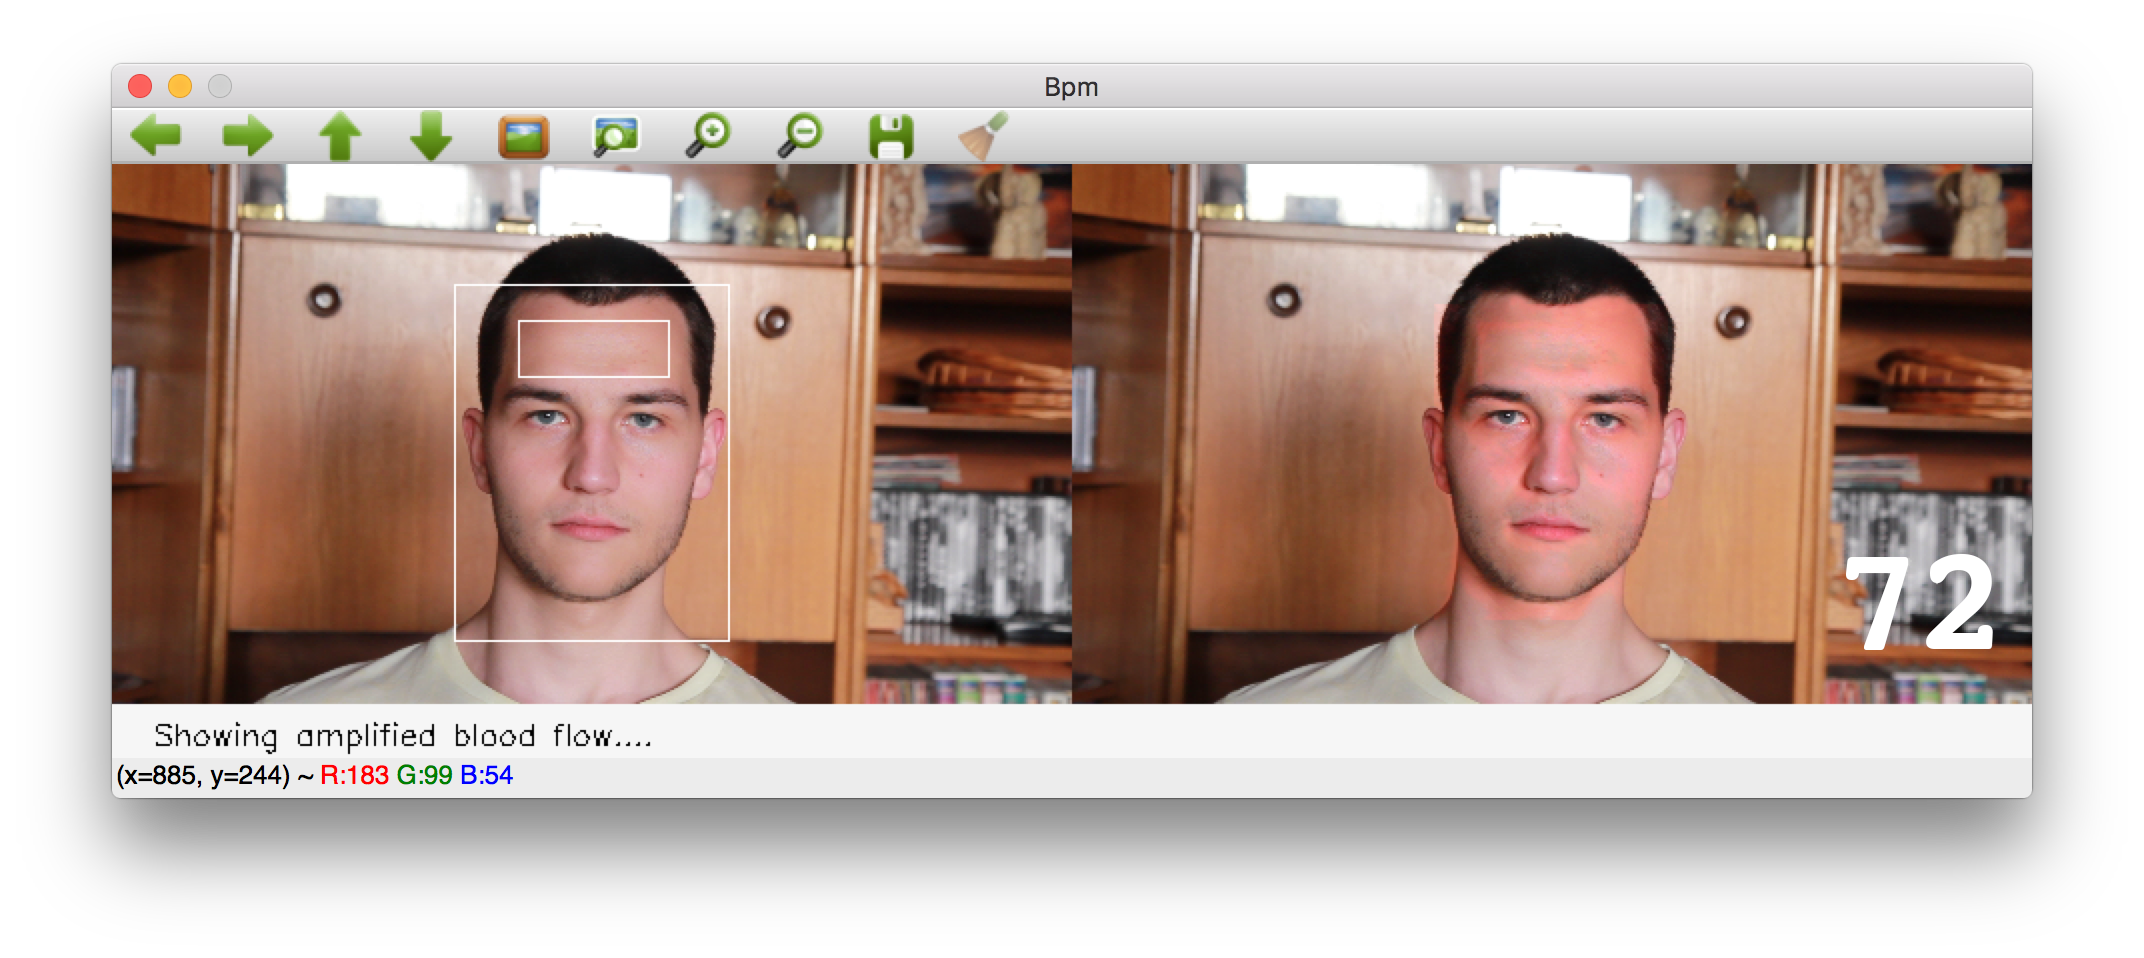
\includegraphics[width=120mm]{images/app-result.png}
  \end{center}
  \caption{Uživatelské rozhraní po dokončení výpočtu tepu i~jeho vizualizace. Vlevo zobrazen aktuální vstupní snímek se zobrazením detekovaného obličeje a čela. Vpravo je zobrazen výsledný snímek s~vizualizací tepu a~s~hodnotou vypočítaného tepu.}
  \label{fig:app-result}
\end{figure}
 
V~bufferu je po celou dobu maximální počet snímků, při vložení snímku nad kapacitu je nejstarší snímek odstraněn. Po dokončení prvního výpočtu aplikace se ihned předává buffer s~novými snímky k~dalšímu zpracování. Opakovaným zpracováním je možné detekovat i~pomalu se měnící tep během snímání. Takto aplikace funguje dokud ji uživatel neukončí. 

\subsection{Rozdíl mezi režimy}
Fungování \emph{reálného} režimu při použití webkamery a~při načteném externím záznamu je velmi podobné. Po vybrání módu se zobrazí okno, kde jsou zobrazeny 2 snímky vedle sebe. Nejdříve budou totožné a po dokončení iniciálního výpočtu jeden slouží pro zobrazení vstupního záznamu a~druhý naopak zobrazuje zpracované snímky.

Jedním z rozdílů mezi \emph{reálným} a \emph{statickým} režimem je ve sběru snímků do bufferu. Zatímco v~\emph{reálném} režimu je zobrazen obraz spolu s~ukládáním snímků do bufferu, ve statickém režimu jsou snímky vloženy do bufferu aniž by bylo původní video viditelné. Pro rychlejší vkládání dat je program vyvíjen ve verzi \emph{OpenCV} s~podporou software \emph{FFmpeg\footnote{FFmpeg je multiplatformní software pro přehrávání, streamování a konvertování videa a zvuku. Dostupné z~\url{https://ffmpeg.org/}}}.

Výpočet tepu je proveden shodným způspobem pro všechny režimy. Při výpočtu vizualizace ve \emph{statickém} režimu je záznam rozdělen na části po 250 snímcích a každá je zpracována ve vlastním vlákně. Toto nastavení velmi zrychluje průběh celého výpočtu.

Odlišně je tvořeno i výstupní video. Díky tomu, že ve \emph{statickém} režimu není při výpočtech nic zobrazeno, aplikace po jeho dokončení může nastavit pozici ve videu zpět na začátek. Proto při kombinaci výstupních snímků vždy snímek z~\emph{vizualizace tepu} odpovídá vstupnímu snímku. Toto není možné při \emph{reálných} režimech, protože by bylo nutné vstup přetáčet. Tím by byla by porušena snaha o~online zpracování, protože by výstupní snímek (časově) neodpovídal vstupnímu.

\section{Měření a požadavky na vstupní záznam}
\label{sec:measure}
Během implementace bylo nutné určit konstanty, které jsou ve výsledné verzi použity. Měření bylo provedeno na mnoha rozdílných záznamech v~rozmezí tepu 58 -- 82 tepů/min. Reálný tep je určen pomocí tlakoměru s~již zmíněnou nepřesností $\pm$ 5\%, proto jsou vypočítané hodnoty tepu spadající do tohoto intervalu považovány za korektní a chyba je udávána až pro hodnoty mimo interval.

% 1. tabulka - roi placement
Nejdříve ukážeme jak je důležité korektně určit masku čela. V~Tabulce \ref{tab:bpm-roi-type} je vidět, že pokus o~určení tepu bez provedení detekce čela je nekorektní především pro situace, kdy je reálný tep vyšší. V~této situaci postup selže jak při použití pouhé masky obličeje, tak při použití celých snímků.

% 2. tabulka - pristup urceni
Další určená hodnota pomocí měření v~Tabulce \ref{tab:bpm-detect-type} je přístup pro tvorbu charakteristických informací o~intenzitách v~každém snímku (popsáno v~kapitole \ref{sec:detect-pulse}). Měření opravdu ukázalo, že se barevné změny nejvíce projevují v~zeleném kanále. Nejpřesnějšího určení tepu je dosaženo s~využitím určování průměrných intenzit hodnot zeleného kanálu, proto bude tento postup nastaven jako výchozí.

% 3. tabulka - delka buffer
Podle provedených měření v~Tabulce \ref{tab:bpm-buffer-frames} byl určen minimální počet snímků pro určení určení tepu na hodnotu \textbf{500} snímků. Tato hodnota odpovídá při vstupní vzorkovací frekvenci 30 snímků/s cca 16 sekundám. Buffer by samozřejmě mohl obsahovat i více snímků, ale pro rychlost zpracování je nutné použít co nejnižší počet snímků.

% FPS
Pro možnost určení tepu je třeba určit i minimální vzorkovací frekvenci. Frekvence obsažené v~záznamu můžeme díky omezení na interval běžného tepu považovat za pásmově omezený. Podle \mbox{Nyquistova} pravidla je určena minimální vzorkovací frekvenci vstupu frekvenci jako dvojnásobek tepové frekvence snímané osoby, neboli:
\begin{equation}
fps_{min} \geq 2*bpm_{real},
\end{equation}
kde $bpm_{real}$ je reálná tepová frekvence. Např. při tepu 60 tepů/min (1 Hz) je potřeba nasnímat záznam minimální vzorkovací frekvencí 2 snímky/s (2 Hz). Toto omezení platí pro samotné určení tepu, nicméně pro uživatele je video už příliš trhané.

% Kdy nefunguje
Určení a vizualizace tepu funguje dobře při denním osvětlení. Během testovacím měření zobrazeném na Obrázku \ref{fig:noise-test} se ukázalo, že postup pro určení tepu není příliš náchylný na šum. Při použití určitého umělého osvětlení na bázi zářivek algoritmus nepracuje příliš dobře i při dostatečném nasvícení. Dá se říci, že je pro aplikaci vhodnější zašumělé video za denního světla než záznam s zářivkovým nasvícením - byť kvalitním.

Největším problémem pro postup je, když se během záznamu obličej příliš hýbá. Takováto videa zpravidla vedou k~nekorektním výsledkům. Bohužel nepomáhá ani stabilizace obrazu před výpočty jak bylo diskutováno v~Kapitole \ref{sec:pulse-detect}.

\begin{figure}
  \begin{center}
    \includegraphics[width=120mm]{images/noise.png}
  \end{center}
  \caption{Na levém snímku je zobrazen snímek z~původního videa. Pro testování je uměle přidáván Gaussovský šum a tep počítán znovu. Na každém snímku je zobrazena standardní odchylka šumu $\sigma$ a výsledný tep $bpm$. I~z~velmi silně zašumělého videa, ilustrovaného pravým snímkem, se podařilo vypočítat tep spadající do korektního intervalu.}
  \label{fig:noise-test}
\end{figure}

V~repositáři je dostupných 20 testovacích z ve složce \textbf{testing}. Pro každé testovací video je vytvořena jedna složka, ve které se nachází:
  \begin{itemize} 
      \item{originální video nazvané podle reálného tepu snímané osoby,}
        \item{výsledné video s~vypočítaným tepem a jeho vizualizací,}
      \item{snímek detekovaného obličeje a čela,}
        \item{textový soubor s~průměrem intenzit zeleného kanálu pro každý snímek použitý pro detekci tepu,}
        \item{ukázku jak ovlivňuje použitá maska čela výsledek,}
        \item{porovnání výsledků při použití různých přístupů z~Kapitoly \ref{sec:detect-pulse} pro určení tepu v~závislosti na počtu použitých snímků v~tabulce ve formátu \emph{.csv}.}
    \end{itemize}

\begin{table}
\label{tab:bpm-detect-type}
\resizebox{\textwidth}{!}{%
\begin{tabular}{@{}rrrrrrr@{}}
\toprule
\textbf{Reálný tep}  & \multicolumn{2}{c}{\textbf{Všechny kanály}} & \multicolumn{2}{c}{\textbf{Zelený kanál}} & \multicolumn{2}{c}{\textbf{Medián zel. kanálu}} \\ \midrule
                    & Výsl. tep                & Chyba {[}\%{]}               & Výsl. tep                 & Chyba {[}\%{]}                 & Výsl. tep            & Chyba {[}\%{]}            \\
58                  & 68                          & 11                           & 61                           & 0                              & 61                      & 0                         \\
60                  & 58                          & 0                            & 58                           & 0                              & 58                      & 0                         \\
62                  & 62                          & 0                            & 68                           & 5                              & 68                      & 5                         \\
66                  & 66                          & 0                            & 66                           & 0                              & 66                      & 0                         \\
68                  & 68                          & 0                            & 68                           & 0                              & 72                      & 0                         \\
70                  & 78                          & 3                            & 78                           & 3                              & 78                      & 3                         \\
72                  & 71                          & 0                            & 71                           & 0                              & 78                      & 3                         \\
73                  & 72                          & 0                            & 75                           & 0                              & 75                      & 0                         \\
81                  & 58                          & 25                           & 83                           & 0                              & 115                     & 35                        \\
82                  & 57                          & 27                           & 87                           & 1                              & 90                      & 5                         \\

Součet chyb &                             & 66                           &                              & 9                              &                         & 51                        \\ \bottomrule
\end{tabular}}
\caption{Výsledky testování rozdílných charakteristik intenzit snímků popsaných v~Kapitole \ref{sec:detect-pulse} pro určení tepu. Ve sloupci \emph{Výsl. tep} je vždy vypočítaný tep aplikací pomocí příslušného přístupu v~hlavičce. V~tomto měření ještě nebyl kladen důraz na výkon aplikace, takže nebylo nutné použít co nejmenší počet snímků pro určení.}
\end{table}

\begin{table}
\label{tab:bpm-roi-type}
\resizebox{\textwidth}{!}{%
\begin{tabular}{rrrr}
\multicolumn{1}{l}{\textbf{Reálný tep záznamu}} & \multicolumn{1}{l}{\textbf{Celý snímek}} & \multicolumn{1}{l}{\textbf{Detekovaný obličej}} & \multicolumn{1}{l}{\textbf{Detekované čelo}} \\
70                                     & 129                             & 129                                    & 78                                  \\
72                                     & 65                              & 65                                     & 72                                  \\
81                                     & 58                              & 58                                     & 83                                  \\
82                                     & 57                              & 57                                     & 87   
\end{tabular}}
\caption{Výsledky ovlivnění výsledků při určení masky pro výpočet intenzit snímků. Princip byl popsán v~Kapitole \ref{sec:detection}. Hodnoty ilustrují situace, kdy je pro výpočet intenzit využit nejdříve celý snímek, potom oblast detekovaného obličeje a nakonec čela.}
\end{table}


\begin{landscape}
\begin{table}
\label{tab:bpm-buffer-frames}
\resizebox{1.5 \textwidth}{!}{%
\begin{tabular}{lllllllllllll}
\toprule
\multicolumn{1}{c}{Reálný tep} & \multicolumn{2}{c}{200 snímků} & \multicolumn{2}{c}{300 snímků} & \multicolumn{2}{c}{400 snímků} & \multicolumn{2}{c}{450 snímků} & \multicolumn{2}{c}{475 snímků} & \multicolumn{2}{c}{500 snímků} \\
                                       & Hodnota    & Chyba {[}\%{]}    & Hodnota    & Chyba {[}\%{]}    & Hodnota    & Chyba {[}\%{]}    & Hodnota    & Chyba {[}\%{]}    & Hodnota    & Chyba {[}\%{]}    & Hodnota    & Chyba {[}\%{]}    \\
58                                     & 72         & 18                & 60         & 0                 & 63         & 3                 & 60         & 0                 & 61         & 0                 & 61         & 0                 \\
60                                     & 63         & 0                 & 60         & 0                 & 59         & 0                 & 60         & 0                 & 61         & 0                 & 58         & 0                 \\
62                                     & 65         & 0                 & 65         & 0                 & 69         & 6                 & 68         & 5                 & 68         & 5                 & 68         & 5                 \\
66                                     & 78         & 13                & 57         & 10                & 74         & 7                 & 73         & 6                 & 72         & 4                 & 66         & 0                 \\
68                                     & 78         & 10                & 73         & 3                 & 74         & 4                 & 73         & 3                 & 72         & 1                 & 66         & 0                 \\
70                                     & 135        & 82                & 130        & 76                & 79         & 7                 & 77         & 4                 & 76         & 3                 & 78         & 5                 \\
72                                     & 79         & 4                 & 72         & 0                 & 72         & 0                 & 71         & 0                 & 71         & 0                 & 72         & 0                 \\
73                                     & 86         & 12                & 77         & 0                 & 76         & 0                 & 74         & 0                 & 73         & 0                 & 75         & 0                 \\
81                                     & 63         & 18                & 60         & 22                & 86         & 1                 & 84         & 0                 & 83         & 0                 & 83         & 0                 \\
82                                     & 60         & 23                & 60         & 23                & 55         & 30                & 56         & 28                & 57         & 27                & 87         & 1                 \\
součet dílčích chyb                    &            & 180               &            & 134               &            & 58                &            & 46                &            & 40                &            & 11               
\end{tabular}}
\caption{Výsledky měření pro určení minimálního počtu snímků pro určení tepu. Pro každý záznam je několikrát určen tep pokaždé s~jiným počtem snímků.}
\end{table}
\end{landscape}


\chapter{Závěr}
Podařilo se vytvořit funkční aplikaci pro detekci a následnou vizualizaci tepu, s možností výběru více režimů. Samotný režim s~využitím webkamery je velice náročný na hardwarové vybavení stroje, na kterém je používán, proto pravděpodobně nebude fungovat na starších hardwarových sestavách. Postup řešení byl obecně velmi náročný na výkon, proto bylo nutné hojně využívat vícevláknové programování pro ulehčení výpočtů. Aplikace umožňuje ve všech režimech uložit výstupní video ve formátu \emph{.avi}.

Při splnění požadavků diskutovaných v~Kapitole \ref{sec:measure} byl u~většiny případů tep určen korektně, s~maximální odchylkou 5\% tepů/min. Detekce tepu nefunguje korektně pro záznamy, v kterých snímaná osoba příliš hýba obličejem, např. při snímání fyzické zátěži. Pro korektní určení tepu je potřeba nejméně 500 snímků, což při vzorkovací frekvenci odpovídá přibližně 17 sekundám, což je doba po kterou je potřeba, aby snímaná osoba co nejméně hýbala obličejem.

Dalším vylepšení do budoucna se nabízí v~řešení problémů příliš velkých pohybů obličeje při snímání, které pv současném stavu končí nekorektním určením tepu. Pro vylepšení vizualizace tepu by bylo možné zpřesnit obdélníkovou masku obličeje přímo na masku obličeje např. pomocí detekce hran a~vizualizaci zobrazovat jen do této masky. Z~hlediska výkonu by bylo možné přesunout část výpočtu na grafickou kartu a~tím celou aplikaci zrychlit, především potom při využití webkamery.


\makeatletter\thesis@blocks@clear\makeatother
\phantomsection %% Print the index and insert it into the
\addcontentsline{toc}{chapter}{\indexname} %% table of contents.
\printindex

\appendix %% Start the appendices.
\chapter{An appendix}
Here you can insert the appendices of your thesis.

\end{document}


